\documentclass[ 12pt ]{article}
\usepackage{amsmath, amsthm, amssymb, enumitem, graphicx, mathrsfs}
\usepackage[margin=0.5in]{geometry}
\graphicspath{ ./ }

\begin{document}

\noindent Landon Fox \\
\noindent Math 486 \\
\noindent September 8, 2020

\begin{center}
\Large Homework 1
\end{center}

\begin{enumerate}
	% problem 1
	\item[\textbf{1.}]
		\begin{enumerate}
			\item[\textbf{1.2.}] Draw a Kuhn tree to math the following verbal description: \\
				\textit{\textbf{The Hidden Pearl}. There are two large drawers, filled with a clutter of miscellanous objects. Player \textbf{i} hides a pearl in one of them. Player
					\textbf{ii} (a burglar?) then has one minute to open a drawer and look for the pearl. If he/she opens Drawer A and the pearl is there, he/she gets it with
					probability $\frac{1}{2}$. If he/she opens Drawer B and the pearl is there, he/she gets it with probability $\frac{1}{3}$. But if he/she opens the wrong drawer they
					get nothing of value.} \\
				Finding the pear is worth +\$50 to \textbf{ii} and -\$50 to \textbf{i}. Failing to find the pearl is worth -\$5 to \textbf{ii} and \$0 to \textbf{i}. \\
				\begin{proof}[Solution]
					The extensive form of the decision problem depicted above.
					\begin{center}
						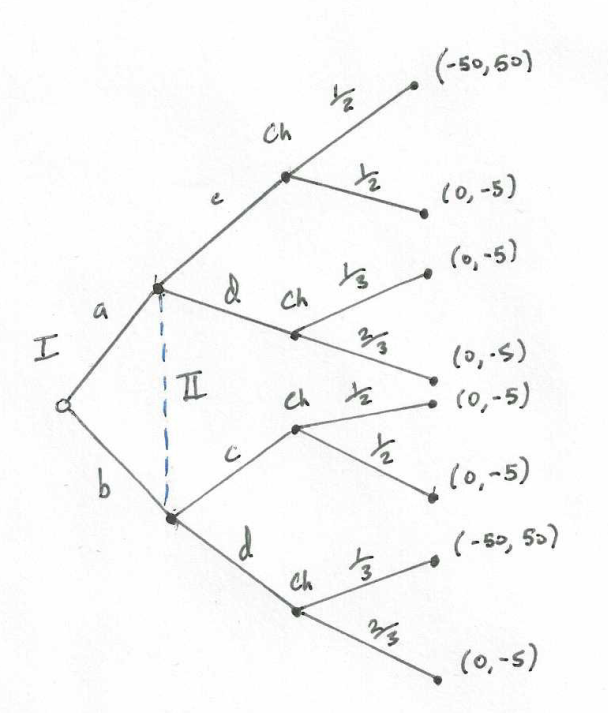
\includegraphics{tree1}
					\end{center}
				\end{proof}
			\newpage


			\item[\textbf{1.3.}] Extend the tree of the pervious exercise to give \textbf{ii} a second chance if he/she did not find the pearl the first time. They may look in the same
				drawer or the other drawer, and the same probabilities and payoffs apply. Note that Player \textbf{i} is not allowed to move the pearl.
				\begin{proof}[Solution]
					The extensive form of the decision problem depicted above.
					\begin{center}
					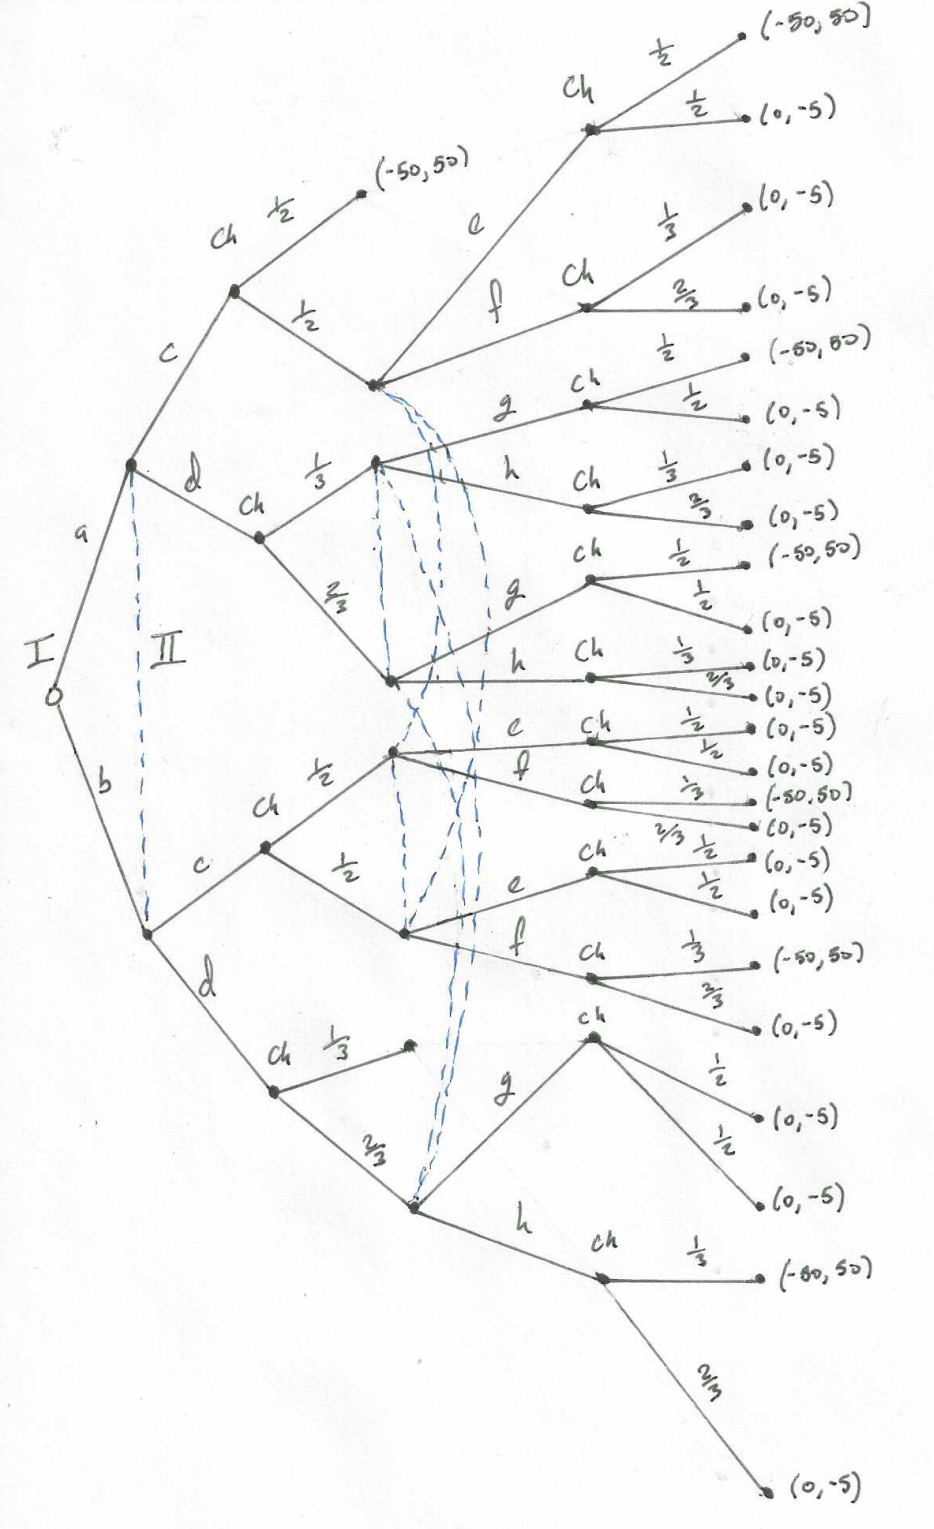
\includegraphics{tree2}
					\end{center}
				\end{proof}
			\newpage


			\item[\textbf{1.4.}]
				Given the verbal description: \\
				\textit{\textbf{The Mutual Admiration Society} is holding its annual Prize Day picnic, at which the entire contents of the treasury will be given to the year's Most
					Admirable member. The winner is determined as follows:}
						\begin{enumerate}
							\item[i.] \textit{The President appoints one of the other members to be the Awards Chair.}
							\item[ii.] \textit{The Awards Chair names one of the other members (but not the President) to be Chief Nominator.}
							\item[iii.] \textit{The Chief Nominator selects one of the remaining members as Most Admirable, and reports back to the Awards Chair.}
							\item[iv.] \textit{The Awards Chair rubberstamps the Chief Nominator's selection, and transmits it to the President.}
							\item[v.] \textit{Finally the President makes a Speech of Admiration to the assembled picnickers and presents the key of the treasury to the incredibly lucky
								winner.}
						\end{enumerate}
						Let there be percisely four members in addition to the President, labeled $A$, $B$, $C$, $D$, and $P$ (the President).
						\newpage
				\begin{enumerate}
					\item[\textbf{1.4a.}] Draw the complete Kuhn tree for this multi-person decision problem. How many terminal nodes are there?
						\begin{proof}[Solution]
							The extensive form of the decision problem depicted above.
							\begin{center}
								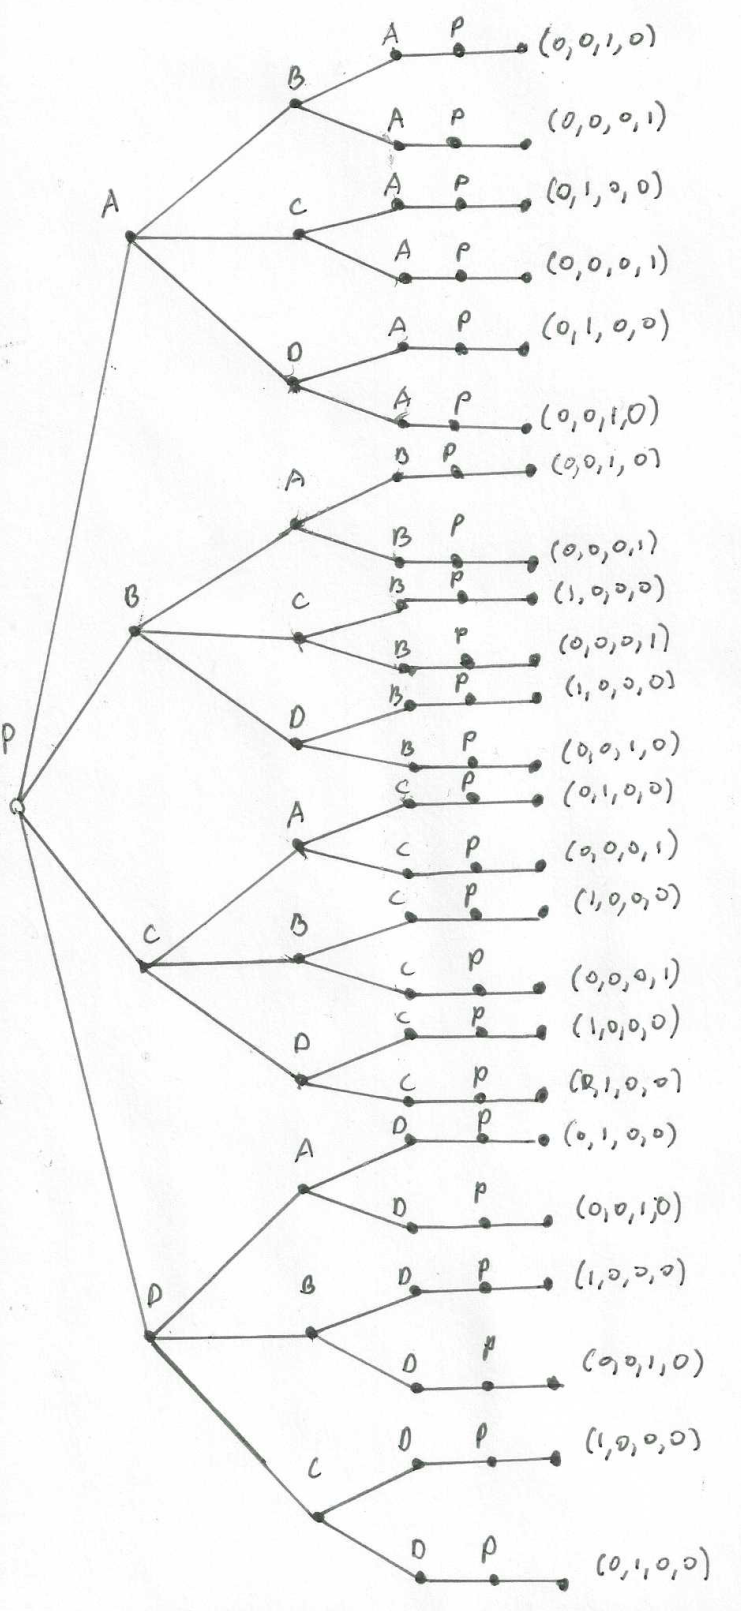
\includegraphics{tree3}
							\end{center}
							After inspection of the tree, we can see that there is exactly 24 terminal nodes.
						\end{proof}
					\newpage

					\item[\textbf{1.4b.}] Suppose the Society has $n \geq 4$ members. Find a formula for the number of terminal nodes. \\
						\begin{proof}[Solution]
							Suppose the Society has $n \geq 4$ members (excluding the President). We can see that therre are three positions to be filled that dictate the extensive form
							of the decision problem. Thus the number of terminal nodes is $n$ permute 3 or $n(n-1)(n-2)$.
						\end{proof}
						
				\end{enumerate}
		\end{enumerate}


	\item[\textbf{2.}]
		\begin{enumerate}
			\item[\textbf{2.1}] For the three person information pattern below, first label all the edges, then list all the full pure strategies and reduced pure strategies.
				\begin{proof}[Solution]
					The extensive form of the provided decision problem.
					\begin{center}
						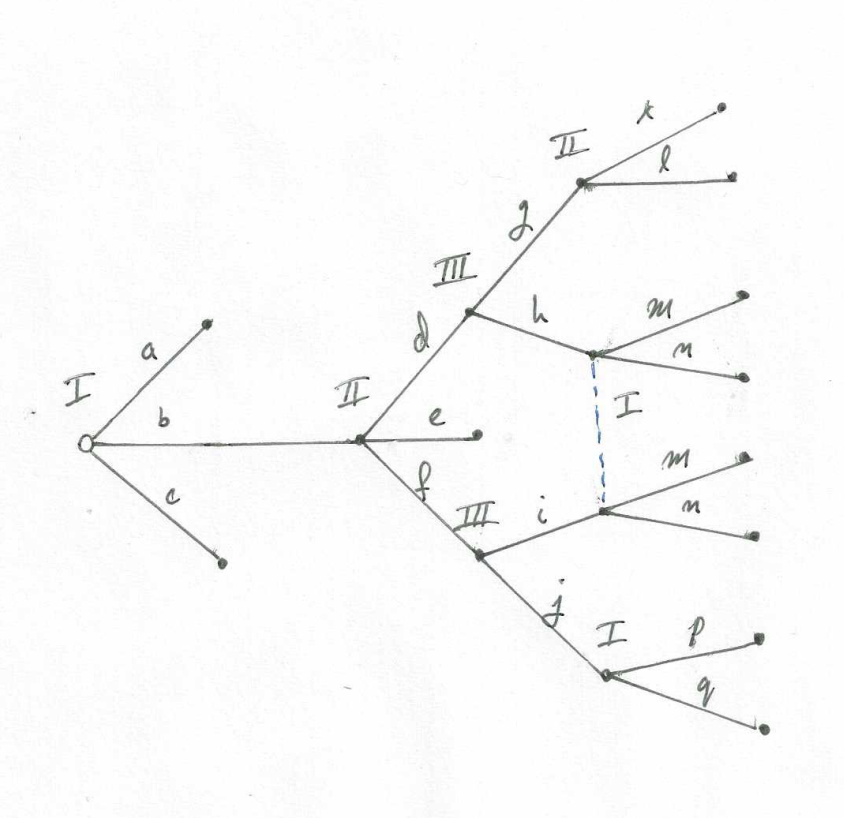
\includegraphics{tree9}
					\end{center}
					Full pure strategies:
					\begin{center}
						\begin{tabular}{|c|c|c|}
							\hline
							\textbf{i} & \textbf{ii} & \textbf{iii} \\
							\hline
							am & dkp & gi \\
							an & dkq & gj \\
							bm & dlp & hi \\
							bn & dlq & hj \\
							cm & ekp & \\
							cn & ekq & \\
							 & elp & \\
							 & elq & \\
							 & fkp & \\
							 & fkq & \\
							 & flp & \\
							 & flq & \\
							\hline
						\end{tabular}
					\end{center}
					\newpage

					Reduced pure strategies:
					\begin{center}
						\begin{tabular}{|c|c|c|}
							\hline
							\textbf{i} & \textbf{ii} & \textbf{iii} \\
							\hline
							a & dk & gi \\
							bm & dl & gj \\
							bn & e & hi \\
							c & fp & hj \\
							 & fq & \\
							\hline
						\end{tabular}
					\end{center}
				\end{proof}

			\item[\textbf{2.1}] Count the pure strategies, full and reduced for each player in the following three person information pattern.
				\begin{center}
					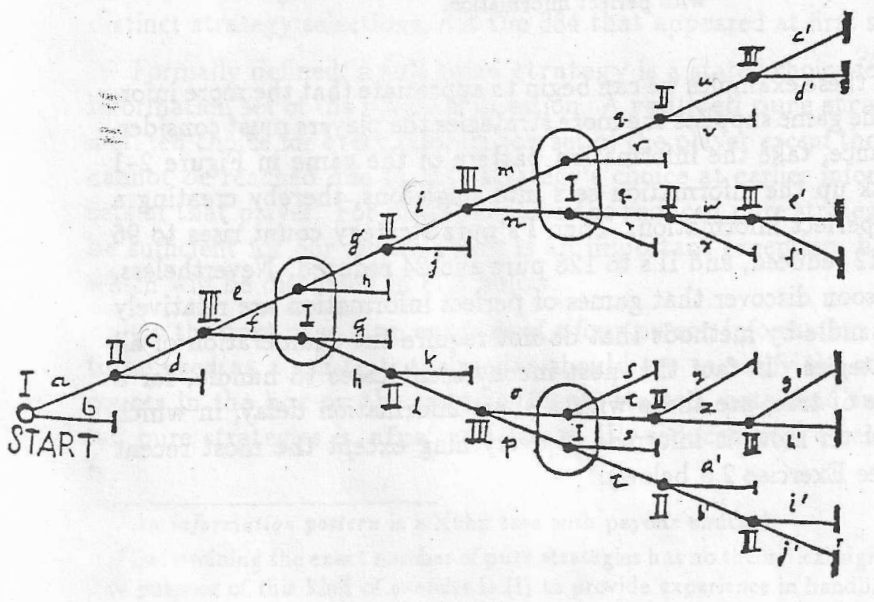
\includegraphics{tree5}
				\end{center}

				\begin{proof}[Solution]
					After inspecting the information sets we can see that there are 16, 128, and 128 full strategies for players \textbf{i}, \textbf{ii}, and \textbf{iii} respectively; additionally,
					there are 5, 26, and 16 reduced strategies for players \textbf{i}, \textbf{ii}, and \textbf{iii} respectively.
				\end{proof}
		\end{enumerate}


	\item[\textbf{3.}]
		\begin{enumerate}
			\item[\textbf{3.1.}] List all the reduced strategies, then reduce the tree to strategic form.
				\begin{center}
					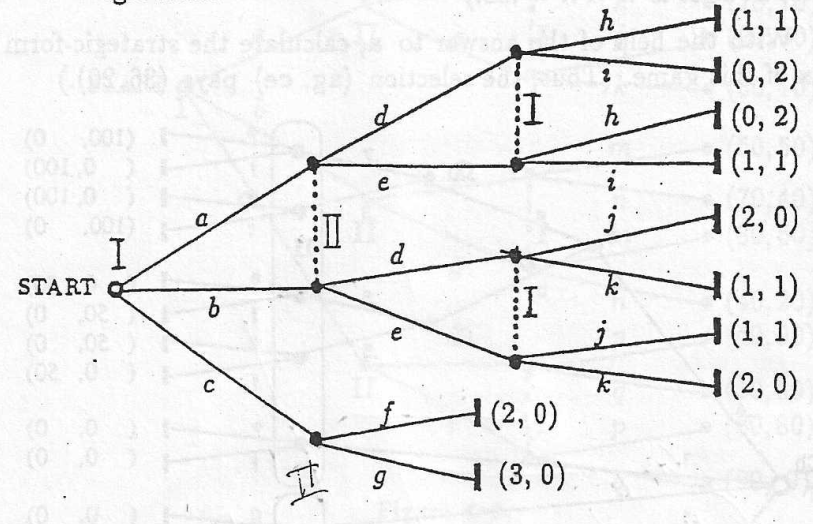
\includegraphics{tree6}
				\end{center}
				\newpage
				\begin{proof}[Solution]
					Reduced pure strategies:
					\begin{center}
						\begin{tabular}{|c|c|}
							\hline
							\textbf{i} & \textbf{ii} \\
							\hline
							ah & df \\
							ai & dg \\
							bj & df \\
							bk & eg \\
							c & \\
							\hline
						\end{tabular}
					\end{center}
					Strategic form:
					\begin{center}
						\begin{tabular}{|c|c|c|c|c|}
							\hline
							i/ii & df & dg & ef & eg \\
							\hline
							ah & (1,1) & (1,1) & (0,2) & (0,2) \\
							ai & (0,2) & (0,2) & (1,1) & (1,1) \\
							bj & (2,0) & (2,0) & (1,1) & (1,1) \\
							bk & (1,1) & (1,1) & (2,0) & (2,0) \\
							c &  (2,0) & (3,0) & (2,0) & (3,0)  \\
							\hline
						\end{tabular}
					\end{center}
				\end{proof}
				
			\item[\textbf{3.2.}] Reduce the following Kuhn tree to strategic form:
				\begin{center}
					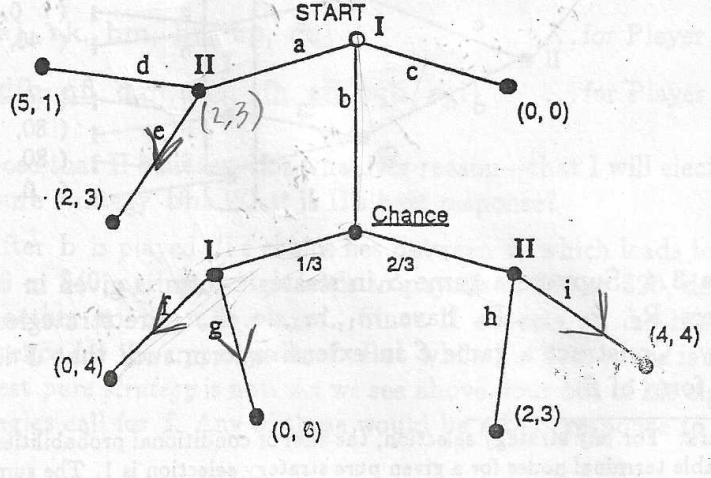
\includegraphics{tree7}
				\end{center}
				\begin{proof}[Solution]
					Strategic form:
					\begin{center}
						\begin{tabular}{|c|c|c|c|c|}
							\hline
							i/ii & di & dh & ei & eh \\
							\hline
							a  & (5,1) & (5,1) & (2,3) & (2,3) \\
							bf & ($\frac{8}{3}$,4) & ($\frac{4}{3}$,$\frac{10}{3}$) & ($\frac{8}{3}$,4) & ($\frac{4}{3}$,$\frac{10}{3}$) \\
							bg & ($\frac{8}{3}$,$\frac{14}{3}$) & ($\frac{4}{3}$,4) & ($\frac{8}{3}$,$\frac{14}{3}$) & ($\frac{4}{3}$,4) \\
							c  & (0,0) & (0,0) & (0,0) & (0,0) \\
							\hline
						\end{tabular}
					\end{center}
				\end{proof}
				\newpage
				
			\item[\textbf{3.3.}] Observe the Kuhn tree below.
				\begin{center}
					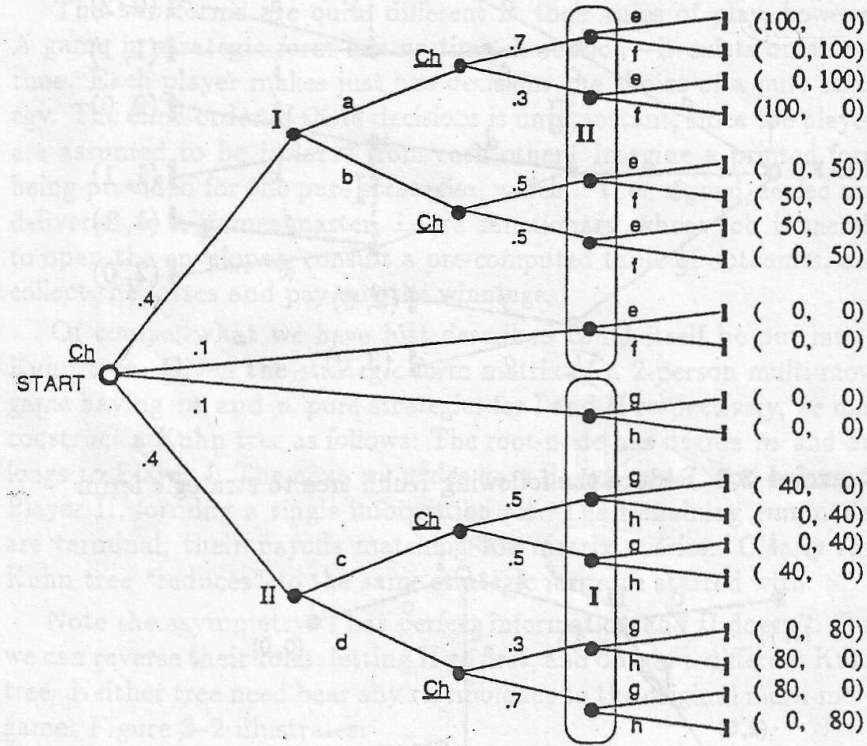
\includegraphics{tree8}
				\end{center}
				\begin{enumerate}
					\item[\textbf{3.3a.}] In the Kuhn tree, determine the conditional probability of each terminal node, assuming that the player's strategy selection has made that node
						attainable.

						\begin{proof}[Solution]
							Listing the probabilities from top to bottom as presented in the Kuhn tree, we have the following:
							\begin{align*}
								&0.28,\; 0.28,\; 0.12,\; 0.12,\; 0.2,\; 0.2,\; 0.2,\; 0.2,\; 0.1,\; 0.1, \\
								&0.1,\; 0.1,\; 0.2,\; 0.2,\; 0.2,\; 0.2,\; 0.12,\; 0.12,\; 0.28,\; 0.28
							\end{align*}
						\end{proof}

					\item[\textbf{3.3b.}] Calculate the strategic form of the presented Kuhn Tree.
						\begin{proof}[Solution]
							Strategic form:
							\begin{center}
								\begin{tabular}{|c|c|c|c|c|}
									\hline
									i/ii   & ce & cf & de & df \\
									\hline
									ag & (36,20) & (20,36) & (50.4,21.6) & (34.4,37.6) \\
									ah & (36,20) & (20,36) & (37.6,34.4) & (21.6,50,4) \\
									bg & (18,18) & (18,18) & (32.4,19.6) & (32.4,19.6) \\
									bh & (18,18) & (18,18) & (19.6,32.4) & (19.6,32.4) \\
									\hline
								\end{tabular}
							\end{center}
						\end{proof}
				\end{enumerate}
			\item[\textbf{4.}] Find all of the Nash Equilibriums of the game in Exercise 3.1.
				\begin{proof}[Solution]
					Strategic form:
					\begin{center}
						\begin{tabular}{|c|c|c|c|c|}
							\hline
							i/ii   & df & dg & ef & eg \\
							\hline
							ah & (1,1) & (1,1) & (0,2)* & (0,2)* \\
							ai & (0,2)* & (0,2)* & (1,1) & (1,1) \\
							bj & *(2,0) & (2,0) & (1,1)* & (1,1)* \\
							bk & (1,1)* & (1,1)* & *(2,0) & (2,0) \\
							c & *(2,0)* & *(3,0)* & *(2,0)* & *(3,0)* \\
							\hline
						\end{tabular}
					\end{center}
					There are four Nash Equilibriums: $\langle c, df \rangle$, $\langle c, dg \rangle$, $\langle c, ef \rangle$, $\langle c, eg \rangle$.
				\end{proof}
				

			\item[\textbf{5.}] Find all of the Nash Equilibriums of the game in Exercise 1.2.
				\begin{proof}[Solution]
					Strategic form:
					\begin{center}
						\begin{tabular}{|c|c|c|}
							\hline
							i/ii   & c & d \\
							\hline
							a & (-25,$\frac{45}{2}$)* & *(0,-5) \\
							b & *(0,-5)* & (-$\frac{50}{3}$, $\frac{40}{3}$)* \\
							\hline
						\end{tabular}
					\end{center}
					There are no Nash Equilibriums.
				\end{proof}
		\end{enumerate}
\end{enumerate}

\end{document}